\documentclass[]{article}
\usepackage{lmodern}
\usepackage{amssymb,amsmath}
\usepackage{ifxetex,ifluatex}
\usepackage{fixltx2e} % provides \textsubscript
\ifnum 0\ifxetex 1\fi\ifluatex 1\fi=0 % if pdftex
  \usepackage[T1]{fontenc}
  \usepackage[utf8]{inputenc}
\else % if luatex or xelatex
  \ifxetex
    \usepackage{mathspec}
  \else
    \usepackage{fontspec}
  \fi
  \defaultfontfeatures{Ligatures=TeX,Scale=MatchLowercase}
  \newcommand{\euro}{€}
\fi
% use upquote if available, for straight quotes in verbatim environments
\IfFileExists{upquote.sty}{\usepackage{upquote}}{}
% use microtype if available
\IfFileExists{microtype.sty}{%
\usepackage{microtype}
\UseMicrotypeSet[protrusion]{basicmath} % disable protrusion for tt fonts
}{}
\usepackage[margin=1in]{geometry}
\usepackage{hyperref}
\PassOptionsToPackage{usenames,dvipsnames}{color} % color is loaded by hyperref
\hypersetup{unicode=true,
            pdfborder={0 0 0},
            breaklinks=true}
\urlstyle{same}  % don't use monospace font for urls
\usepackage{color}
\usepackage{fancyvrb}
\newcommand{\VerbBar}{|}
\newcommand{\VERB}{\Verb[commandchars=\\\{\}]}
\DefineVerbatimEnvironment{Highlighting}{Verbatim}{commandchars=\\\{\}}
% Add ',fontsize=\small' for more characters per line
\usepackage{framed}
\definecolor{shadecolor}{RGB}{248,248,248}
\newenvironment{Shaded}{\begin{snugshade}}{\end{snugshade}}
\newcommand{\KeywordTok}[1]{\textcolor[rgb]{0.13,0.29,0.53}{\textbf{{#1}}}}
\newcommand{\DataTypeTok}[1]{\textcolor[rgb]{0.13,0.29,0.53}{{#1}}}
\newcommand{\DecValTok}[1]{\textcolor[rgb]{0.00,0.00,0.81}{{#1}}}
\newcommand{\BaseNTok}[1]{\textcolor[rgb]{0.00,0.00,0.81}{{#1}}}
\newcommand{\FloatTok}[1]{\textcolor[rgb]{0.00,0.00,0.81}{{#1}}}
\newcommand{\ConstantTok}[1]{\textcolor[rgb]{0.00,0.00,0.00}{{#1}}}
\newcommand{\CharTok}[1]{\textcolor[rgb]{0.31,0.60,0.02}{{#1}}}
\newcommand{\SpecialCharTok}[1]{\textcolor[rgb]{0.00,0.00,0.00}{{#1}}}
\newcommand{\StringTok}[1]{\textcolor[rgb]{0.31,0.60,0.02}{{#1}}}
\newcommand{\VerbatimStringTok}[1]{\textcolor[rgb]{0.31,0.60,0.02}{{#1}}}
\newcommand{\SpecialStringTok}[1]{\textcolor[rgb]{0.31,0.60,0.02}{{#1}}}
\newcommand{\ImportTok}[1]{{#1}}
\newcommand{\CommentTok}[1]{\textcolor[rgb]{0.56,0.35,0.01}{\textit{{#1}}}}
\newcommand{\DocumentationTok}[1]{\textcolor[rgb]{0.56,0.35,0.01}{\textbf{\textit{{#1}}}}}
\newcommand{\AnnotationTok}[1]{\textcolor[rgb]{0.56,0.35,0.01}{\textbf{\textit{{#1}}}}}
\newcommand{\CommentVarTok}[1]{\textcolor[rgb]{0.56,0.35,0.01}{\textbf{\textit{{#1}}}}}
\newcommand{\OtherTok}[1]{\textcolor[rgb]{0.56,0.35,0.01}{{#1}}}
\newcommand{\FunctionTok}[1]{\textcolor[rgb]{0.00,0.00,0.00}{{#1}}}
\newcommand{\VariableTok}[1]{\textcolor[rgb]{0.00,0.00,0.00}{{#1}}}
\newcommand{\ControlFlowTok}[1]{\textcolor[rgb]{0.13,0.29,0.53}{\textbf{{#1}}}}
\newcommand{\OperatorTok}[1]{\textcolor[rgb]{0.81,0.36,0.00}{\textbf{{#1}}}}
\newcommand{\BuiltInTok}[1]{{#1}}
\newcommand{\ExtensionTok}[1]{{#1}}
\newcommand{\PreprocessorTok}[1]{\textcolor[rgb]{0.56,0.35,0.01}{\textit{{#1}}}}
\newcommand{\AttributeTok}[1]{\textcolor[rgb]{0.77,0.63,0.00}{{#1}}}
\newcommand{\RegionMarkerTok}[1]{{#1}}
\newcommand{\InformationTok}[1]{\textcolor[rgb]{0.56,0.35,0.01}{\textbf{\textit{{#1}}}}}
\newcommand{\WarningTok}[1]{\textcolor[rgb]{0.56,0.35,0.01}{\textbf{\textit{{#1}}}}}
\newcommand{\AlertTok}[1]{\textcolor[rgb]{0.94,0.16,0.16}{{#1}}}
\newcommand{\ErrorTok}[1]{\textcolor[rgb]{0.64,0.00,0.00}{\textbf{{#1}}}}
\newcommand{\NormalTok}[1]{{#1}}
\usepackage{graphicx,grffile}
\makeatletter
\def\maxwidth{\ifdim\Gin@nat@width>\linewidth\linewidth\else\Gin@nat@width\fi}
\def\maxheight{\ifdim\Gin@nat@height>\textheight\textheight\else\Gin@nat@height\fi}
\makeatother
% Scale images if necessary, so that they will not overflow the page
% margins by default, and it is still possible to overwrite the defaults
% using explicit options in \includegraphics[width, height, ...]{}
\setkeys{Gin}{width=\maxwidth,height=\maxheight,keepaspectratio}
\setlength{\parindent}{0pt}
\setlength{\parskip}{6pt plus 2pt minus 1pt}
\setlength{\emergencystretch}{3em}  % prevent overfull lines
\providecommand{\tightlist}{%
  \setlength{\itemsep}{0pt}\setlength{\parskip}{0pt}}
\setcounter{secnumdepth}{0}

%%% Use protect on footnotes to avoid problems with footnotes in titles
\let\rmarkdownfootnote\footnote%
\def\footnote{\protect\rmarkdownfootnote}

%%% Change title format to be more compact
\usepackage{titling}

% Create subtitle command for use in maketitle
\newcommand{\subtitle}[1]{
  \posttitle{
    \begin{center}\large#1\end{center}
    }
}

\setlength{\droptitle}{-2em}
  \title{}
  \pretitle{\vspace{\droptitle}}
  \posttitle{}
  \author{}
  \preauthor{}\postauthor{}
  \date{}
  \predate{}\postdate{}


% Redefines (sub)paragraphs to behave more like sections
\ifx\paragraph\undefined\else
\let\oldparagraph\paragraph
\renewcommand{\paragraph}[1]{\oldparagraph{#1}\mbox{}}
\fi
\ifx\subparagraph\undefined\else
\let\oldsubparagraph\subparagraph
\renewcommand{\subparagraph}[1]{\oldsubparagraph{#1}\mbox{}}
\fi

\usepackage{ctex} 
\setCJKmainfont{宋体}                     % 中文缺省字体,
\setCJKsansfont{黑体}                      % 中文无衬线字体,   调用命令: \sffamily
\setCJKmonofont{仿宋}     % 中文打字机(等宽)字体, 调用命令: \ttfamily

%\usepackage{ctex} 
%\setCJKmainfont{Adobe 宋体 Std}                     % 中文缺省字体,
%\setCJKsansfont{Adobe 黑体 Std}                      % 中文无衬线字体,   调用命令: \sffamily
%\setCJKmonofont{Adobe 仿宋 Std}     % 中文打字机(等宽)字体, 调用命令: \ttfamily

\begin{document}

\subsection{经济系 何友鑫 15320161152320}\label{--15320161152320}

\subsection{R Code}\label{r-code}

\begin{Shaded}
\begin{Highlighting}[]
\NormalTok{filename <-}\StringTok{ }\KeywordTok{dir}\NormalTok{(}\StringTok{"./Data/"}\NormalTok{)}
\CommentTok{#删除隐藏文件}
\NormalTok{filename <-}\StringTok{ }\NormalTok{filename[-(}\DecValTok{1}\NormalTok{:}\DecValTok{6}\NormalTok{)]}
\NormalTok{price_plot <-}\StringTok{ }\NormalTok{function(}\DataTypeTok{flag=}\DecValTok{0}\NormalTok{,i)}
\NormalTok{\{}
  \NormalTok{filepath <-}\StringTok{ }\KeywordTok{paste0}\NormalTok{(}\StringTok{"./Data/"}\NormalTok{,filename[i])}
  \NormalTok{if(flag==}\DecValTok{0}\NormalTok{)}
  \NormalTok{\{}
    \CommentTok{#从第三部分开始读取文件,即28行开始}
    \NormalTok{file <-}\StringTok{ }\KeywordTok{read.xlsx}\NormalTok{(filepath,}\DecValTok{1}\NormalTok{,}\DataTypeTok{startRow =} \DecValTok{28}\NormalTok{)}
  \NormalTok{\}}
  \NormalTok{if(flag==}\DecValTok{1}\NormalTok{)}
  \NormalTok{\{}
    \CommentTok{#问题3的第三部分数据是从33行开始}
    \NormalTok{file <-}\StringTok{ }\KeywordTok{read.xlsx}\NormalTok{(filepath,}\DecValTok{1}\NormalTok{,}\DataTypeTok{startRow =} \DecValTok{33}\NormalTok{)}
  \NormalTok{\}}
  \CommentTok{#tradeID=0,-1的行剔除 按tradeID升序排列}
  \NormalTok{file <-}\StringTok{ }\KeywordTok{filter}\NormalTok{(file,tradeID>}\DecValTok{0}\NormalTok{)}
  \NormalTok{file <-}\StringTok{ }\NormalTok{file[}\KeywordTok{order}\NormalTok{(file$tradeID),]}
  
  \NormalTok{group1 <-}\StringTok{ }\KeywordTok{filter}\NormalTok{(file,Group==}\DecValTok{1}\NormalTok{)}
  \CommentTok{#time_t <- c(1:nrow(group1))}
  \NormalTok{title <-}\StringTok{ }\KeywordTok{paste0}\NormalTok{(filename[i],}\StringTok{"_group1 price"}\NormalTok{)}
  \NormalTok{plot1 <-}\StringTok{ }\KeywordTok{ggplot}\NormalTok{(group1,}\KeywordTok{aes}\NormalTok{(}\DataTypeTok{x=}\NormalTok{group1$tradeID,group1$price))+}
\StringTok{    }\KeywordTok{geom_line}\NormalTok{(}\DataTypeTok{colour=}\StringTok{"green"}\NormalTok{)+}
\StringTok{    }\KeywordTok{ggtitle}\NormalTok{(title)}
  \KeywordTok{print}\NormalTok{(plot1)}
 
  \NormalTok{group2 <-}\StringTok{ }\KeywordTok{filter}\NormalTok{(file,Group==}\DecValTok{2}\NormalTok{)}
  \CommentTok{#time_t <- c(1:nrow(group2))}
  \NormalTok{title <-}\StringTok{ }\KeywordTok{paste0}\NormalTok{(filename[i],}\StringTok{"_group2 price"}\NormalTok{)}
  \NormalTok{plot2 <-}\StringTok{ }\KeywordTok{ggplot}\NormalTok{(group2,}\KeywordTok{aes}\NormalTok{(}\DataTypeTok{x=}\NormalTok{group2$tradeID,group2$price))+}
\StringTok{    }\KeywordTok{geom_line}\NormalTok{(}\DataTypeTok{colour=}\StringTok{"red"}\NormalTok{)+}
\StringTok{    }\KeywordTok{ggtitle}\NormalTok{(title)}
  \KeywordTok{print}\NormalTok{(plot2)}
\NormalTok{\}}
\end{Highlighting}
\end{Shaded}

\subsection{\texorpdfstring{Q1.第一场至第七场``可融资实验''第一轮}{Q1.第一场至第七场可融资实验第一轮}}\label{q1.}

\begin{Shaded}
\begin{Highlighting}[]
\NormalTok{for (i in }\DecValTok{1}\NormalTok{:}\DecValTok{7}\NormalTok{) }
\NormalTok{\{}
  \KeywordTok{price_plot}\NormalTok{(}\DecValTok{0}\NormalTok{,i)}
\NormalTok{\}}
\end{Highlighting}
\end{Shaded}

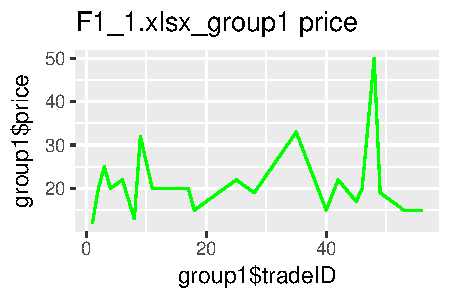
\includegraphics{finance_homework_files/figure-latex/unnamed-chunk-3-1.pdf}
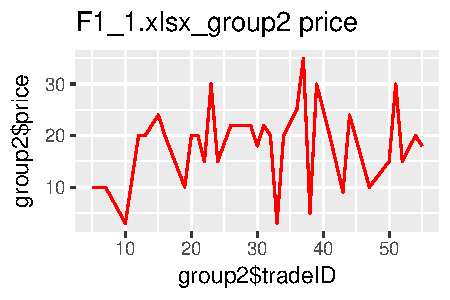
\includegraphics{finance_homework_files/figure-latex/unnamed-chunk-3-2.pdf}
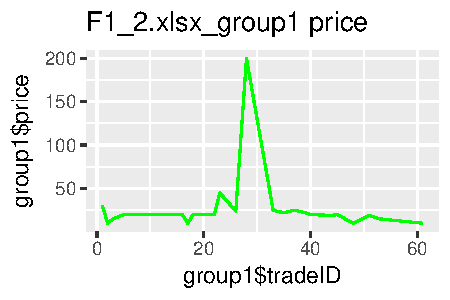
\includegraphics{finance_homework_files/figure-latex/unnamed-chunk-3-3.pdf}
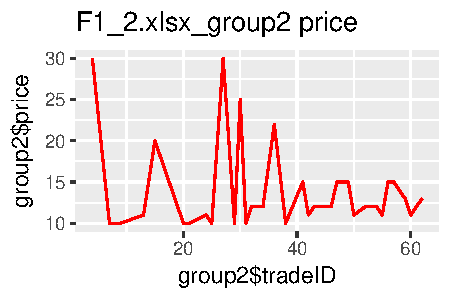
\includegraphics{finance_homework_files/figure-latex/unnamed-chunk-3-4.pdf}
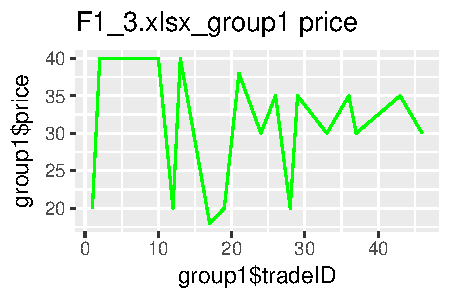
\includegraphics{finance_homework_files/figure-latex/unnamed-chunk-3-5.pdf}
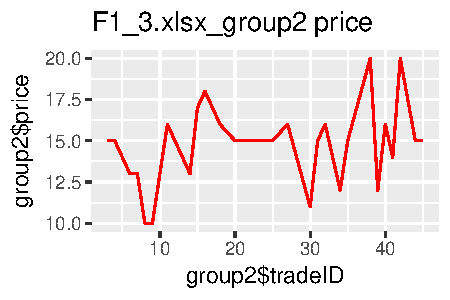
\includegraphics{finance_homework_files/figure-latex/unnamed-chunk-3-6.pdf}
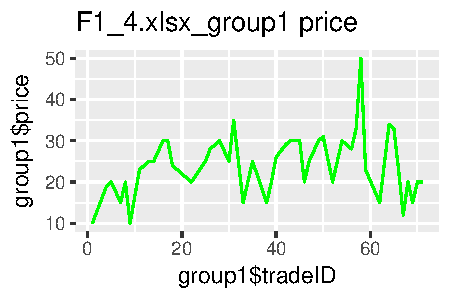
\includegraphics{finance_homework_files/figure-latex/unnamed-chunk-3-7.pdf}
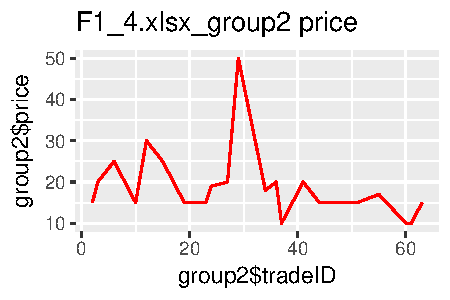
\includegraphics{finance_homework_files/figure-latex/unnamed-chunk-3-8.pdf}
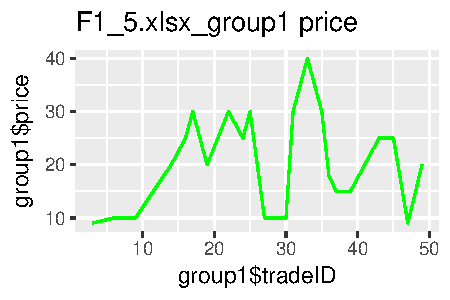
\includegraphics{finance_homework_files/figure-latex/unnamed-chunk-3-9.pdf}
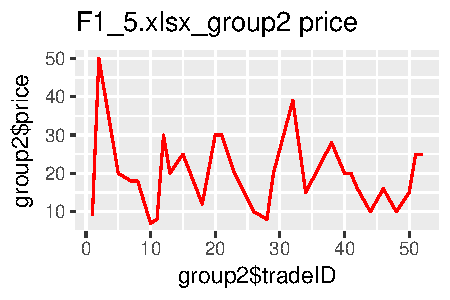
\includegraphics{finance_homework_files/figure-latex/unnamed-chunk-3-10.pdf}
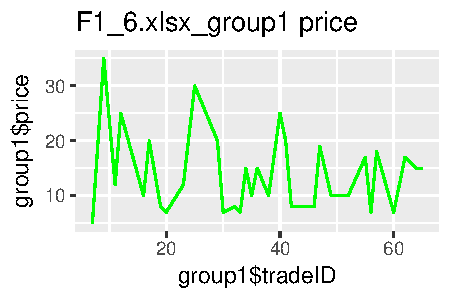
\includegraphics{finance_homework_files/figure-latex/unnamed-chunk-3-11.pdf}
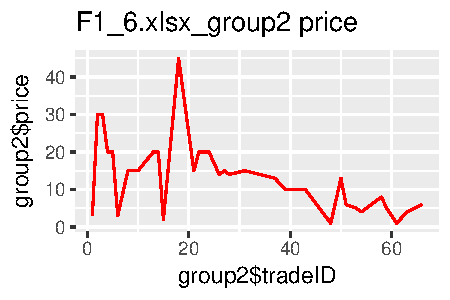
\includegraphics{finance_homework_files/figure-latex/unnamed-chunk-3-12.pdf}
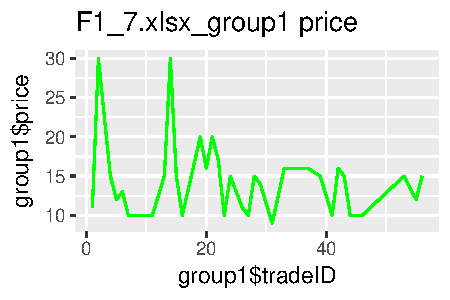
\includegraphics{finance_homework_files/figure-latex/unnamed-chunk-3-13.pdf}
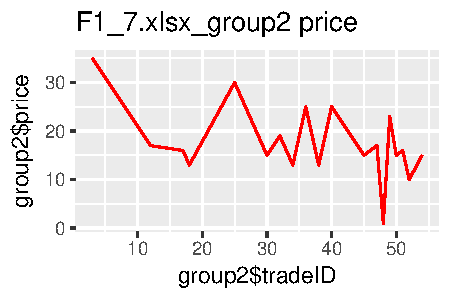
\includegraphics{finance_homework_files/figure-latex/unnamed-chunk-3-14.pdf}

\newpage

\subsection{\texorpdfstring{Q2.第一场至第七场``不可融资实验''第一轮}{Q2.第一场至第七场不可融资实验第一轮}}\label{q2.}

\begin{Shaded}
\begin{Highlighting}[]
\NormalTok{for (i in }\DecValTok{27}\NormalTok{:}\DecValTok{33}\NormalTok{) }
\NormalTok{\{}
  \KeywordTok{price_plot}\NormalTok{(}\DecValTok{0}\NormalTok{,i)}
\NormalTok{\}}
\end{Highlighting}
\end{Shaded}

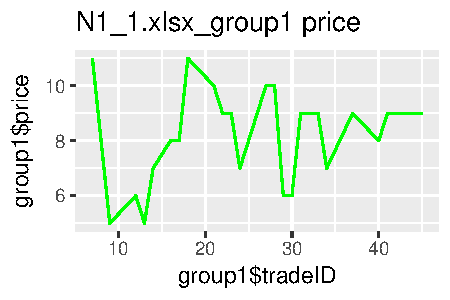
\includegraphics{finance_homework_files/figure-latex/unnamed-chunk-4-1.pdf}
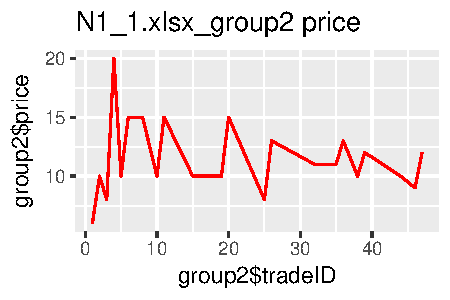
\includegraphics{finance_homework_files/figure-latex/unnamed-chunk-4-2.pdf}
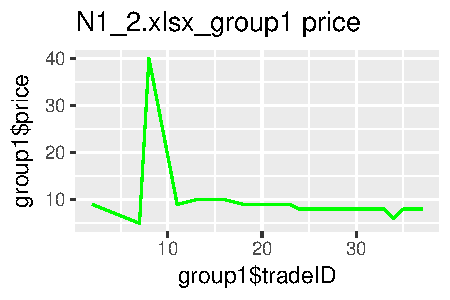
\includegraphics{finance_homework_files/figure-latex/unnamed-chunk-4-3.pdf}
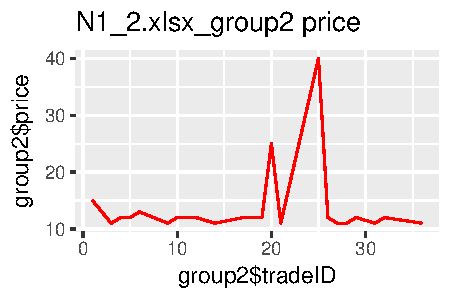
\includegraphics{finance_homework_files/figure-latex/unnamed-chunk-4-4.pdf}
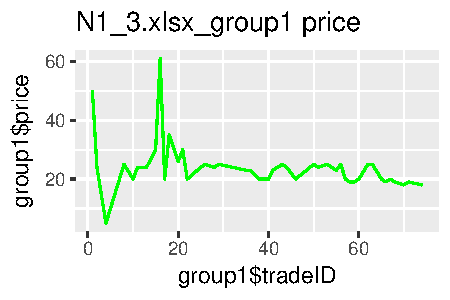
\includegraphics{finance_homework_files/figure-latex/unnamed-chunk-4-5.pdf}
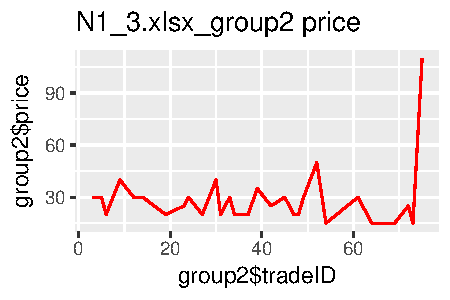
\includegraphics{finance_homework_files/figure-latex/unnamed-chunk-4-6.pdf}
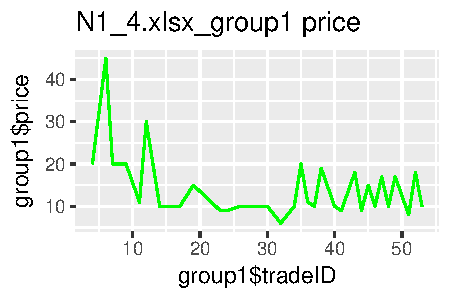
\includegraphics{finance_homework_files/figure-latex/unnamed-chunk-4-7.pdf}
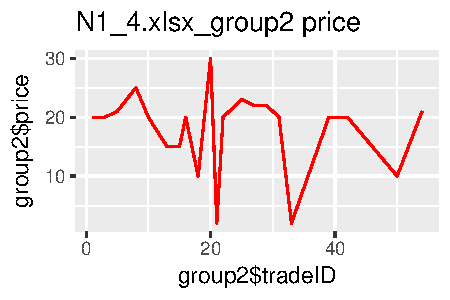
\includegraphics{finance_homework_files/figure-latex/unnamed-chunk-4-8.pdf}
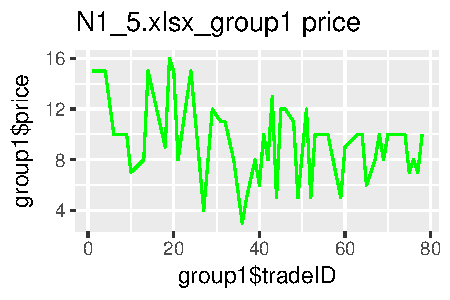
\includegraphics{finance_homework_files/figure-latex/unnamed-chunk-4-9.pdf}
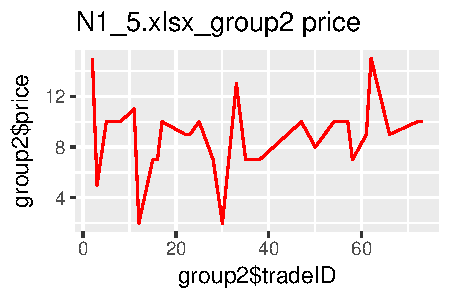
\includegraphics{finance_homework_files/figure-latex/unnamed-chunk-4-10.pdf}
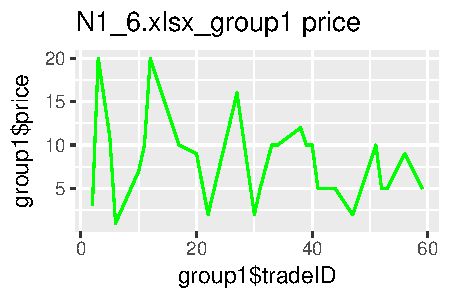
\includegraphics{finance_homework_files/figure-latex/unnamed-chunk-4-11.pdf}
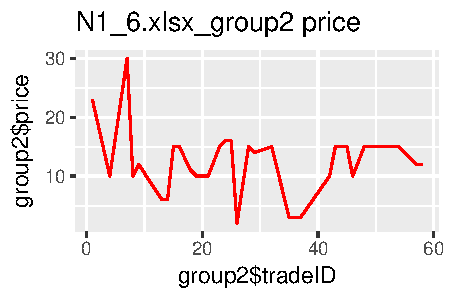
\includegraphics{finance_homework_files/figure-latex/unnamed-chunk-4-12.pdf}
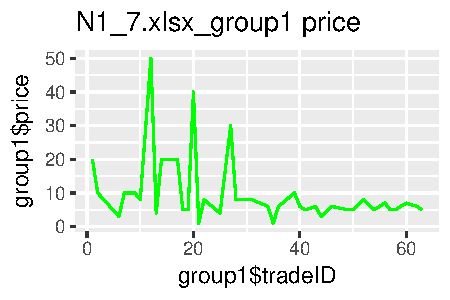
\includegraphics{finance_homework_files/figure-latex/unnamed-chunk-4-13.pdf}
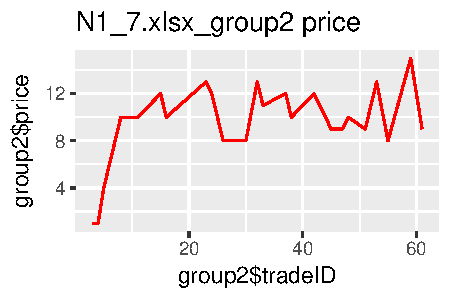
\includegraphics{finance_homework_files/figure-latex/unnamed-chunk-4-14.pdf}

\newpage

\subsection{\texorpdfstring{Q3.第一场至第七场``可融资实验''第四轮}{Q3.第一场至第七场可融资实验第四轮}}\label{q3.}

\begin{Shaded}
\begin{Highlighting}[]
\NormalTok{for (i in }\DecValTok{22}\NormalTok{:}\DecValTok{26}\NormalTok{) }
\NormalTok{\{}
  \KeywordTok{price_plot}\NormalTok{(}\DecValTok{1}\NormalTok{,i)}
\NormalTok{\}}
\end{Highlighting}
\end{Shaded}

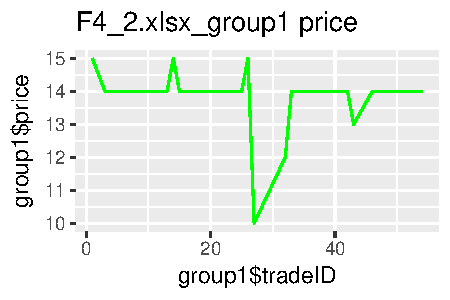
\includegraphics{finance_homework_files/figure-latex/unnamed-chunk-5-1.pdf}
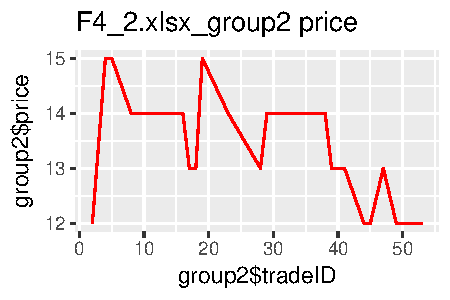
\includegraphics{finance_homework_files/figure-latex/unnamed-chunk-5-2.pdf}
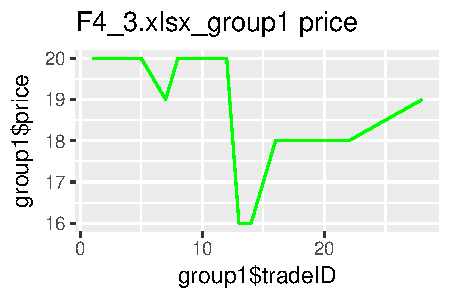
\includegraphics{finance_homework_files/figure-latex/unnamed-chunk-5-3.pdf}
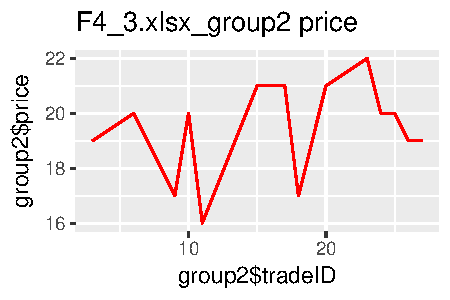
\includegraphics{finance_homework_files/figure-latex/unnamed-chunk-5-4.pdf}
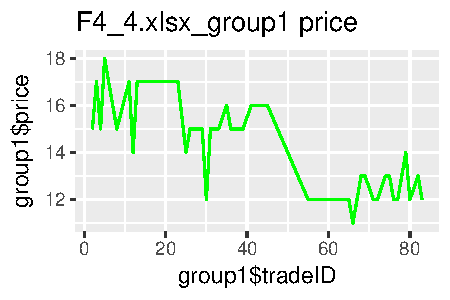
\includegraphics{finance_homework_files/figure-latex/unnamed-chunk-5-5.pdf}
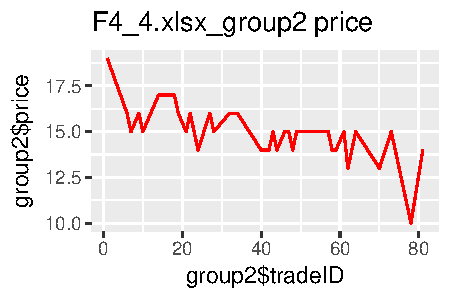
\includegraphics{finance_homework_files/figure-latex/unnamed-chunk-5-6.pdf}
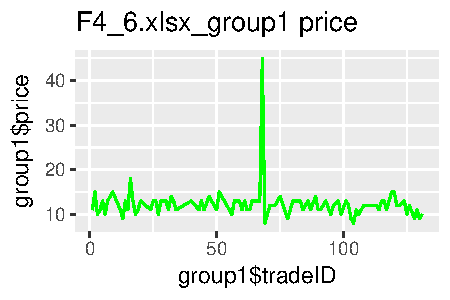
\includegraphics{finance_homework_files/figure-latex/unnamed-chunk-5-7.pdf}
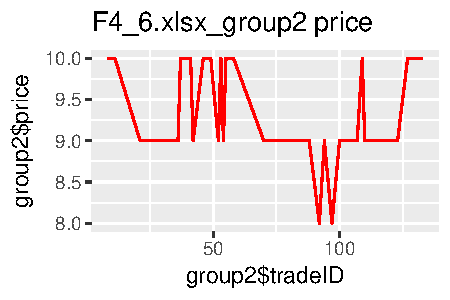
\includegraphics{finance_homework_files/figure-latex/unnamed-chunk-5-8.pdf}
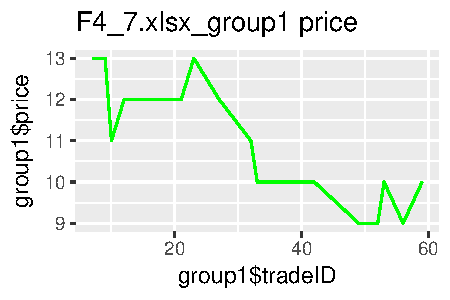
\includegraphics{finance_homework_files/figure-latex/unnamed-chunk-5-9.pdf}
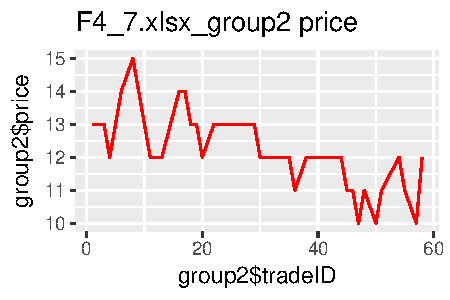
\includegraphics{finance_homework_files/figure-latex/unnamed-chunk-5-10.pdf}

\newpage

\subsection{Q4.}\label{q4.}

\subsubsection{1.相对于可融资实验,不可融资实验中游戏资产交易价格的波动幅度更小。}

\subsubsection{2.从交易价格的极端值来看,可融资交易出现了一次200元,四次50元,而不可融资交易相对应的是一次150元,一次60元,一次50元。}\label{200501506050}

\subsection{Q5.}\label{q5.}

\subsubsection{第四轮交易手数多,交易更为频繁,价格波动快。}

\subsection{Q6.}\label{q6.}

\subsubsection{1.共谋的方式:资产高价成交,把资金转移到一个人手里。}

\subsubsection{2.防止合谋的方法:1)将每个交易者隔绝,禁止私下接触;2)每一场比赛每一轮重新分配每一组的交易对手。确保每一场交易中交易者都面临不同的交易对手。3)设置涨跌停。}\label{123}

\subsection{Q7.}\label{q7.}

\subsubsection{1.参与者面临的随机性不够。表现在12个交易对手确定为一个小组后,此后的几轮交易没有变更小组成员,而且一些小组成员互相认识,在同一个地方交易,提高了合谋的可能性。}\label{12}

\subsubsection{2.针对资产的最终价值的确定,随机数设置不合理,资产价值可能为0也可能很高。这增加了实验的投机性,并不利于探讨现实中投资者的面临不确定风险下的选择。建议提高资产价值的下限。}\label{0}

\subsubsection{3.最终收益率的确定应该看四轮交易的平均值而不是随机抽取一轮。否则会促使交易者进行更加非理性的决策。}

\subsection{Q8.}\label{q8.}

\subsubsection{无关。根据实验数据分析可得,initial money 与 final payoff
、return rate
无直接联系。}\label{initial-money--final-payoff-return-rate-}

\subsection{Q9.}\label{q9.}

\subsubsection{1.每轮的交易时间太短,有时市场很不活跃。}

\subsubsection{2.在实验中,作空更容易得到高收益。}

\subsubsection{3.投资者易采取极端手段获取高收益,有存在高价(异常)价格成交的数据,说明在实验中存在
共谋。}\label{-}

\subsubsection{4.实验者参与者以咖啡卷为目的,不以盈利为目的,是非理性人。}

\subsubsection{5.资产真实价格的分布不太合理。}

\end{document}
